\chapter{Data Structures}

The NTP state machines are defined in the following sections. State
variables are separated into classes according to their function in
packet headers, peer and poll processes, the system process, and the
clock discipline process. Packet variables represent the NTP header
values in transmitted and received packets. Peer and poll variables
represent the contents of the association for each server separately.
System variables represent the state of the server as seen by its
dependent clients. Clock discipline variables represent the internal
workings of the clock discipline algorithm. An example is described
in Appendix A.

\section{Structure Conventions}

In order to distinguish between different variables of the same name
but used in different processes, the naming convention summarized in
Figure 5 is adopted. A receive packet variable v is a member of the
packet structure r with fully qualified name r.v. In a similar
manner, x.v is a transmit packet variable, p.v is a peer variable,
s.v is a system variable, and c.v is a clock discipline variable.
There is a set of peer variables for each association; there is only
one set of system and clock variables.

\begin{table}[htb]
\center
\begin{tabular}{c | c | c}
Name & Description \\
\hline
\hline
r. & receive packet header variable \\
x. & transmit packet header variable \\
p. & peer/poll variable \\
s. & system variable \\
c. & clock discipline variable \\
\hline
\end{tabular}
\label{prefix_conventions}
\caption{Prefix Conventions}
\end{table}

\section{Global Parameters}

In addition to the variable classes, a number of global parameters
are defined in this document, including those shown with values in
Figure 6.

\begin{table}[htb]
\center
\begin{tabular}{c | c | c}
Name & Value & Description \\
\hline
\hline
PORT & 123 & NTP port number \\
VERSION & 4 & NTP version number \\
TOLERANCE & 15e-6 & frequency tolerance PHI (s/s) \\
MINPOLL & 4 & minimum poll exponent (16 s) \\
MAXPOLL & 17 & maximum poll exponent (36 h) \\
MAXDISP & 16 & maximum dispersion (16 s) \\
MINDISP & .005 & minimum dispersion increment (s) \\
MAXDIST & 1 & distance threshold (1 s) \\
MAXSTRAT & 16 & maximum stratum number \\
\hline
\end{tabular}
\label{global_parameters}
\caption{Global Parameters}
\end{table}

While these are the only global parameters needed for
interoperability, a larger collection is necessary in any
implementation. Appendix A.1.1 contains those used by the skeleton
for the mitigation algorithms, clock discipline algorithm, and
related implementation-dependent functions. Some of these parameter
values are cast in stone, like the NTP port number assigned by the
IANA and the version number assigned NTPv4 itself. Others, like the
frequency tolerance (also called PHI), involve an assumption about
the worst-case behavior of a system clock once synchronized and then
allowed to drift when its sources have become unreachable. The
minimum and maximum parameters define the limits of state variables
as described in later sections of this document.

While shown with fixed values in this document, some implementations
may make them variables adjustable by configuration commands. For
instance, the reference implementation computes the value of
PRECISION as log2 of the minimum time in several iterations to read
the system clock.

\section{Packet Header Variables}

The most important state variables from an external point of view are
the packet header variables described in Figure 7 and below. The NTP
packet header consists of an integral number of 32-bit (4 octet)
words in network byte order. The packet format consists of three
components: the header itself, one or more optional extension fields,
and an optional message authentication code (MAC). The header
component is identical to the NTPv3 header and previous versions.
The optional extension fields are used by the Autokey public key
cryptographic algorithms described in \cite{RFC5906}. The optional MAC is
used by both Autokey and the symmetric key cryptographic algorithm
described in this RFC.

\begin{table}[htb]
\center
\begin{tabular}{c | c | c}
Name & Formula & Description \\
\hline
\hline
leap & leap & leap indicator (LI) \\
version & version & version number (VN) \\
mode & mode & mode \\
stratum & stratum & stratum \\
poll & poll & poll exponent \\
precision & rho & precision exponent \\
rootdelay & delta\_r & root delay \\
rootdisp & epsilon\_r & root dispersion \\
refid & refid & reference ID \\
reftime & reftime & reference timestamp \\
org & T1 & origin timestamp \\
rec & T2 & receive timestamp \\
xmt & T3 & transmit timestamp \\
dst & T4 & destination timestamp \\
keyid & keyid & key ID \\
dgst & dgst & message digest \\
\hline
\end{tabular}
\label{packet_header_variables}
\caption{Packet Header Variables}
\end{table}

The NTP packet is a UDP datagram \cite{RFC0768}. Some fields use multiple
words and others are packed in smaller fields within a word. The NTP
packet header shown in Figure 8 has 12 words followed by optional
extension fields and finally an optional message authentication code
(MAC) consisting of the Key Identifier field and Message Digest
field.

\begin{figure}
\centering
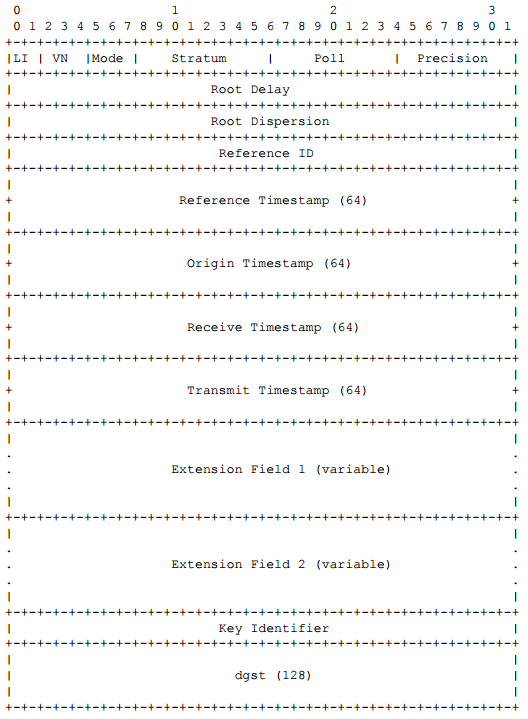
\includegraphics[width=\textwidth]{packet_header_format.png}
\caption{Packet Header Format}
\label{packet_header_format}
\end{figure}

The extension fields are used to add optional capabilities, for
example, the Autokey security protocol [RFC5906]. The extension
field format is presented in order for the packet to be parsed
without the knowledge of the extension field functions. The MAC is
used by both Autokey and the symmetric key authentication scheme.

A list of the packet header variables is shown in Figure 7 and
described in detail below. Except for a minor variation when using
the IPv6 address family, these fields are backwards compatible with
NTPv3. The packet header fields apply to both transmitted packets (x
prefix) and received packets (r prefix). In Figure 8, the size of
some multiple-word fields is shown in bits if not the default 32
bits. The basic header extends from the beginning of the packet to
the end of the Transmit Timestamp field.

The fields and associated packet variables (in parentheses) are
interpreted as follows:

\begin{description}

\item[LI Leap Indicator (leap)] 2-bit integer warning of an impending leap
second to be inserted or deleted in the last minute of the current
month with values defined in Figure 9.

\begin{table}[htb]
\center
\begin{tabular}{c | c | c}
Value & Meaning \\
\hline
\hline
0 & no warning \\
1 & last minute of the day has 61 seconds \\
2 & last minute of the day has 59 seconds \\
3 & unknown (clock unsynchronized) \\
\hline
\end{tabular}
\label{leap_indicator}
\caption{Leap Indicator}
\end{table}

\item[VN Version Number (version)] 3-bit integer representing the NTP
version number, currently 4.

\item[Mode (mode)] 3-bit integer representing the mode, with values defined
in Figure 10.

\begin{table}[htb]
\center
\begin{tabular}{c | c | c}
Value & Meaning \\
\hline
\hline
0 & reserved \\
1 & symmetric active \\
2 & symmetric passive \\
3 & client \\
4 & server \\
5 & broadcast \\
6 & NTP control message \\
7 & reserved for private use \\
\hline
\end{tabular}
\label{association_modes}
\caption{Association Modes}
\end{table}

\item[Stratum (stratum)] 8-bit integer representing the stratum, with
values defined in Figure 11.

\begin{table}[htb]
\center
\begin{tabular}{c | c | c}
Value & Meaning \\
\hline
\hline
0 & unspecified or invalid \\
1 & primary server (e.g., equipped with a GPS receiver) \\
2-15 & secondary server (via NTP) \\
16 & unsynchronized \\
17-255 & reserved \\
\hline
\end{tabular}
\label{packet_stratum}
\caption{Packet Stratum}
\end{table}

It is customary to map the stratum value 0 in received packets to
MAXSTRAT (16) in the peer variable p.stratum and to map p.stratum
values of MAXSTRAT or greater to 0 in transmitted packets. This
allows reference clocks, which normally appear at stratum 0, to be
conveniently mitigated using the same clock selection algorithms used
for external sources (see Appendix A.5.5.1 for an example).

\item[Poll] 8-bit signed integer representing the maximum interval between
successive messages, in log2 seconds. Suggested default limits for
minimum and maximum poll intervals are 6 and 10, respectively.

\item[Precision] 8-bit signed integer representing the precision of the
system clock, in log2 seconds. For instance, a value of -18
corresponds to a precision of about one microsecond. The precision
can be determined when the service first starts up as the minimum
time of several iterations to read the system clock.

\item[Root Delay (rootdelay)] Total round-trip delay to the reference
clock, in NTP short format.

\item[Root Dispersion (rootdisp)] Total dispersion to the reference clock,
in NTP short format.

\item[Reference ID (refid)] 32-bit code identifying the particular server
or reference clock. The interpretation depends on the value in the
stratum field. For packet stratum 0 (unspecified or invalid), this
is a four-character ASCII \ref{RFC1345} string, called the "kiss code",
used for debugging and monitoring purposes. For stratum 1 (reference
clock), this is a four-octet, left-justified, zero-padded ASCII
string assigned to the reference clock. The authoritative list of
Reference Identifiers is maintained by IANA; however, any string
beginning with the ASCII character "X" is reserved for unregistered
experimentation and development. The identifiers in Figure 12 have
been used as ASCII identifiers:

\begin{table}[htb]
\center
\begin{tabular}{c | c | c}
ID & Clock Source \\
\hline
\hline
GOES & Geosynchronous Orbit Environment Satellite \\
GPS & Global Position System \\
GAL & Galileo Positioning System \\
PPS & Generic pulse-per-second \\
IRIG & Inter-Range Instrumentation Group \\
WWVB & LF Radio WWVB Ft. Collins, CO 60 kHz \\
DCF & LF Radio DCF77 Mainflingen, DE 77.5 kHz \\
HBG & LF Radio HBG Prangins, HB 75 kHz \\
MSF & LF Radio MSF Anthorn, UK 60 kHz \\
JJY & LF Radio JJY Fukushima, JP 40 kHz, Saga, JP 60 kHz \\
LORC & MF Radio LORAN C station, 100 kHz \\
TDF & MF Radio Allouis, FR 162 kHz \\
CHU & HF Radio CHU Ottawa, Ontario \\
WWV & HF Radio WWV Ft. Collins, CO \\
WWVH & HF Radio WWVH Kauai, HI \\
NIST & NIST telephone modem \\
ACTS & NIST telephone modem \\
USNO & USNO telephone modem \\
PTB & European telephone modem \\
\hline
\end{tabular}
\label{reference_identifiers}
\caption{Reference Identifiers}
\end{table}

\item[Above stratum 1 (secondary servers and clients)] this is the
reference identifier of the server and can be used to detect timing
loops. If using the IPv4 address family, the identifier is the four-
octet IPv4 address. If using the IPv6 address family, it is the
first four octets of the MD5 hash of the IPv6 address. Note that,
when using the IPv6 address family on an NTPv4 server with a NTPv3
client, the Reference Identifier field appears to be a random value
and a timing loop might not be detected.

\item[Reference Timestamp] Time when the system clock was last set or
corrected, in NTP timestamp format.

\item[Origin Timestamp (org)] Time at the client when the request departed
for the server, in NTP timestamp format.

\item[Receive Timestamp (rec)] Time at the server when the request arrived
from the client, in NTP timestamp format.

\item[Transmit Timestamp (xmt)] Time at the server when the response left
for the client, in NTP timestamp format.

\item[Destination Timestamp (dst)] Time at the client when the reply
arrived from the server, in NTP timestamp format.

Note: The Destination Timestamp field is not included as a header
field; it is determined upon arrival of the packet and made available
in the packet buffer data structure.

If the NTP has access to the physical layer, then the timestamps are
associated with the beginning of the symbol after the start of frame.
Otherwise, implementations should attempt to associate the timestamp
to the earliest accessible point in the frame.

The MAC consists of the Key Identifier followed by the Message
Digest. The message digest, or cryptosum, is calculated as in
\cite{RFC1321} over all NTP-header and optional extension fields, but not
the MAC itself.

\item[Extension Field n] See Section 7.5 for a description of the format of
this field.

\item[Key Identifier (keyid)] 32-bit unsigned integer used by the client
and server to designate a secret 128-bit MD5 key.

\item[Message Digest (digest)] 128-bit MD5 hash computed over the key
followed by the NTP packet header and extensions fields (but not the
Key Identifier or Message Digest fields).

\end{description}

It should be noted that the MAC computation used here differs from
those defined in \cite{RFC1305} and \cite{RFC4330} but is consistent with how
existing implementations generate a MAC.

\section{The Kiss-o’-Death Packet}

If the Stratum field is 0, which implies unspecified or invalid, the
Reference Identifier field can be used to convey messages useful for
status reporting and access control. These are called Kiss-o’-Death
(KoD) packets and the ASCII messages they convey are called kiss
codes. The KoD packets got their name because an early use was to
tell clients to stop sending packets that violate server access
controls. The kiss codes can provide useful information for an
intelligent client, either NTPv4 or SNTPv4. Kiss codes are encoded
in four-character ASCII strings that are left justified and zero
filled. The strings are designed for character displays and log
files. A list of the currently defined kiss codes is given in
Figure 13. Recipients of kiss codes MUST inspect them and, in the
following cases, take these actions:

\begin{enumerate}[a.]
  \item For kiss codes DENY and RSTR, the client MUST demobilize any
associations to that server and stop sending packets to that
server;
  \item For kiss code RATE, the client MUST immediately reduce its
polling interval to that server and continue to reduce it each
time it receives a RATE kiss code.
  \item Kiss codes beginning with the ASCII character "X" are for
unregistered experimentation and development and MUST be ignored
if not recognized.
  \item Other than the above conditions, KoD packets have no protocol
significance and are discarded after inspection.
\end{enumerate}

\begin{table}[htb]
\center
\begin{tabular}{c | c | c}
Code & Meaning \\
\hline
\hline
ACST & The association belongs to a unicast server. \\
AUTH & Server authentication failed. \\
AUTO & Autokey sequence failed. \\
BCST & The association belongs to a broadcast server. \\
CRYP & Cryptographic authentication or identification failed. \\
DENY & Access denied by remote server. \\
DROP & Lost peer in symmetric mode. \\
RSTR & Access denied due to local policy. \\
INIT & The association has not yet synchronized for the first time. \\
MCST & The association belongs to a dynamically discovered server.\\
NKEY & No key found. Either the key was never installed or is not trusted. \\
RATE & Rate exceeded. The server has temporarily denied access because the client exceeded the rate threshold. \\
RMOT & Alteration of association from a remote host running ntpdc. \\
STEP & A step change in system time has occurred, but the association has not yet resynchronized. \\
\hline
\end{tabular}
\label{kiss_codes}
\caption{Kiss Codes}
\end{table}

The Receive Timestamp and the Transmit Timestamp (set by the server)
are undefined when in a KoD packet and MUST NOT be relied upon to
have valid values and MUST be discarded.

\section{NTP Extension Field Format}

In NTPv4, one or more extension fields can be inserted after the
header and before the MAC, which is always present when an extension
field is present. Other than defining the field format, this
document makes no use of the field contents. An extension field
contains a request or response message in the format shown in
Figure 14.

\begin{figure}
\centering
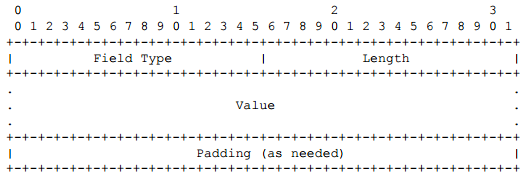
\includegraphics[width=\textwidth]{extension_field_format.png}
\caption{Extension Field Format}
\label{extension_field_format}
\end{figure}

All extension fields are zero-padded to a word (four octets)
boundary. The Field Type field is specific to the defined function
and is not elaborated here. While the minimum field length
containing required fields is four words (16 octets), a maximum field
length remains to be established.

The Length field is a 16-bit unsigned integer that indicates the
length of the entire extension field in octets, including the Padding
field.
